\documentclass[12pt, oneside, a4paper]{report}
\usepackage{hyperref,graphicx}
\usepackage[top=3cm, bottom=3cm, left=3cm, right=3cm]{geometry}
\usepackage{setspace}
\usepackage{fontspec}
\usepackage{float}
\usepackage{color}
\usepackage[usenames,dvipsnames,svgnames,table]{xcolor}
\usepackage{xunicode}
\usepackage{array}
\usepackage{booktabs,bookmark}
\usepackage{longtable}
\usepackage{ragged2e}
\usepackage[font={footnotesize,it}]{caption}
\usepackage{parskip}
\usepackage{amsmath}
\usepackage{amssymb}
\usepackage{bm}
\usepackage{textcomp}
%\usepackage[customcolors]{hf-tikz}
\usepackage{xspace}
\usepackage[Greek,Latin]{ucharclasses}
\usepackage{xltxtra}
\usepackage{xgreek} 
\usepackage[sort&compress,numbers]{natbib}
\usepackage{float}
\usepackage{mathtools}

% \usepackage[utf8]{inputenc}

%\usepackage{minted}

\renewcommand{\labelenumii}{\theenumii}
\renewcommand{\theenumii}{\theenumi.\arabic{enumii}.}

%\floatname{algorithm}{Αλγόριθμος}
\renewcommand\figurename{Εικόνα}
%\renewcommand\tablename{Πίνακας}

\setTransitionsForGreek{\setlanguage{greek}}{\setlanguage{american}} % Instead of american, any other language can be used

\renewcommand\thesection{\arabic{section}}

\hypersetup{
 %bookmarks=true, % show bookmarks bar?
unicode=true, % non-Latin characters in Acrobat’s bookmarks
pdftoolbar=true, % show Acrobat’s toolbar?
pdfmenubar=true, % show Acrobat’s menu?
pdffitwindow=false, % window fit to page when opened
pdfstartview={FitH}, % fits the width of the page to the window
pdftitle={Stakeholder's Requirements Specification}, % title
pdfauthor={Daphne Tsolissou}, % author
pdfsubject={}, % subject of the document
pdfcreator={LaTeX}, % creator of the document
% pdfproducer={LateX}, % producer of the document
%pdfkeywords= % list of keywords
pdfnewwindow=true, % links in new window
colorlinks=false, % false: boxed links; true: colored links
linkbordercolor={1 1 1}, % color of internal links (change box color with linkbordercolor)
%citecolor=white, % color of links to bibliography
citebordercolor={1 1 1},
filecolor=magenta, % color of file links
urlcolor=cyan % color of external links
}

\setmainfont{Times New Roman}
\singlespacing
\frenchspacing
\setlength{\parindent}{0.6cm}
\setlength{\parskip}{0.5pt}

\begin{document}
%      \parbox[l]{\textwidth}{
\flushleft{\Huge{\textbf{Έγγραφο απαιτήσεων εμπλεκομένων μερών (StRS)}}}\\
\flushleft{\Huge{\textbf{Stakeholders Requirements Specification}}}\\
\flushleft{\footnotesize{ΠΡΟΣΑΡΜΟΓΗ ΤΟΥ ΑΝΤΙΣΤΟΙΧΟΥ ΕΓΓΡΑΦΟΥ ΤΟΥ ΠΡΟΤΥΠΟΥ ISO/IEC/IEEE 29148:2011}}\\
    \vspace{1cm}
\flushleft{\Large{\textbf{Software Developers}}}\\
    \vspace{1cm}

\pagestyle{plain}
\pagenumbering{arabic}
\normalsize
\section{Εισαγωγή}

\subsection{Ταυτότητα-επιχειρησιακοί στόχοι}
\hspace{0.6cm}Ως εταιρεία κατασκευής λογισμικού έχουμε σαν στόχο να αναπτύξουμε ένα σύστημα παρατηρητηριού τιμών συσκευών κινητής τηλεφωνίας το οποίο θα ανταποκρίνεται στις απαιτήσεις των εμπλεκόμενων μερών του έργου όπως ορίζονται στα αντίστοιχα έγγραφα. Μετά την υλοποίηση του συστήματος θα συνεχίσουμε να το υποστηρίζουμε και να το συντηρούμε καθ'όλη τη διάρκεια ζωής του. 

\hspace{0.6cm}Για την μελλοντική διαχείριση του συστήματος από εγγεκριμένα άτομα θα υλοποιηθεί κατάλληλο περιβάλλον όπου θα μπορούν να κάνουν εργασίες στο backend κομμάτι. Αυτό θα επιταχύνει και διευκολύνει το να γίνονται κοινές διαχειριστικές λειτουργίες που διαφορετικά θα χρειάζονταν κόπο και χρόνο.

\subsection{Περίγραμμα επιχειρησιακών λειτουργιών}

\hspace{0.6cm}Ο διαχειριστής είναι ένας τύπος χρήστη που παίζει καθοριστικό ρόλο όσον αφορά την ασφάλεια και την ομαλή λειτουργία του συστήματος και έχει απόλυτη ελευθερία σχετικά με την επεξεργασία και τη διαχείρισή του. 

\hspace{0.6cm}Ένας από τους ρόλους εξέχουσας σημασίας ενός διαχειριστή είναι να κρίνει αν οι εθελοντές-χρήστες είναι αξιόπιστοι ελέγχοντας τις τιμές που συμπληρώνουν σε κάθε πεδίο (π.χ. αν υπάρχει το όνομα καταστήματος, το όνομα του προϊόντος, αν η τιμή είναι εξωφρενικά μεγάλη για συγκεκριμένο προϊόν). Έτσι, αν κάποιος εθελοντής είναι αξιόπιστος θα συνεχίζει κανονικά να καταχωρεί προϊόντα, ενώ σε αντίθετη περίπτωση θα αναστέλλεται αυτή του η δυνατότητα.

\hspace{0.6cm}Θα μπορεί, επιπροσθέτως, να έχει πρόσβαση στους λογαριασμούς των χρηστών όπου και θα μπορεί να επεξεργάζεται τα προφίλ τους για να αλλάζει τα δικαιώματα και τους ρόλους των χρηστών, μέσα από συγκεκριμένη σελίδα. Ο τρόπος που προστατεύεται η πλατφόρμα είναι επιτρέποντας μόνο σε χρήστες με δικαιώματα διαχειριστή να μπορούν να κάνουν τροποποιήσεις σε αρχεία ή εφαρμογές.

\hspace{0.6cm}Για να τα πραγματοποιήσει όλα αυτά του παρέχεται ξεχωριστός λογαριασμός διαχειριστή με δυνατότητα αναζήτησης χρηστών, πρόσβαση στις πληροφορίες των λογαριασμών τους και δυνατότητα επεξεργασίας τους.

\hspace{0.6cm}Στην εικόνα \ref{uml2} φαίνεται το use-case uml διάγραμμα της αλληλεπίδρασης του διαχειριστή με το σύστημα.

\begin{figure}[H]
   \centering
   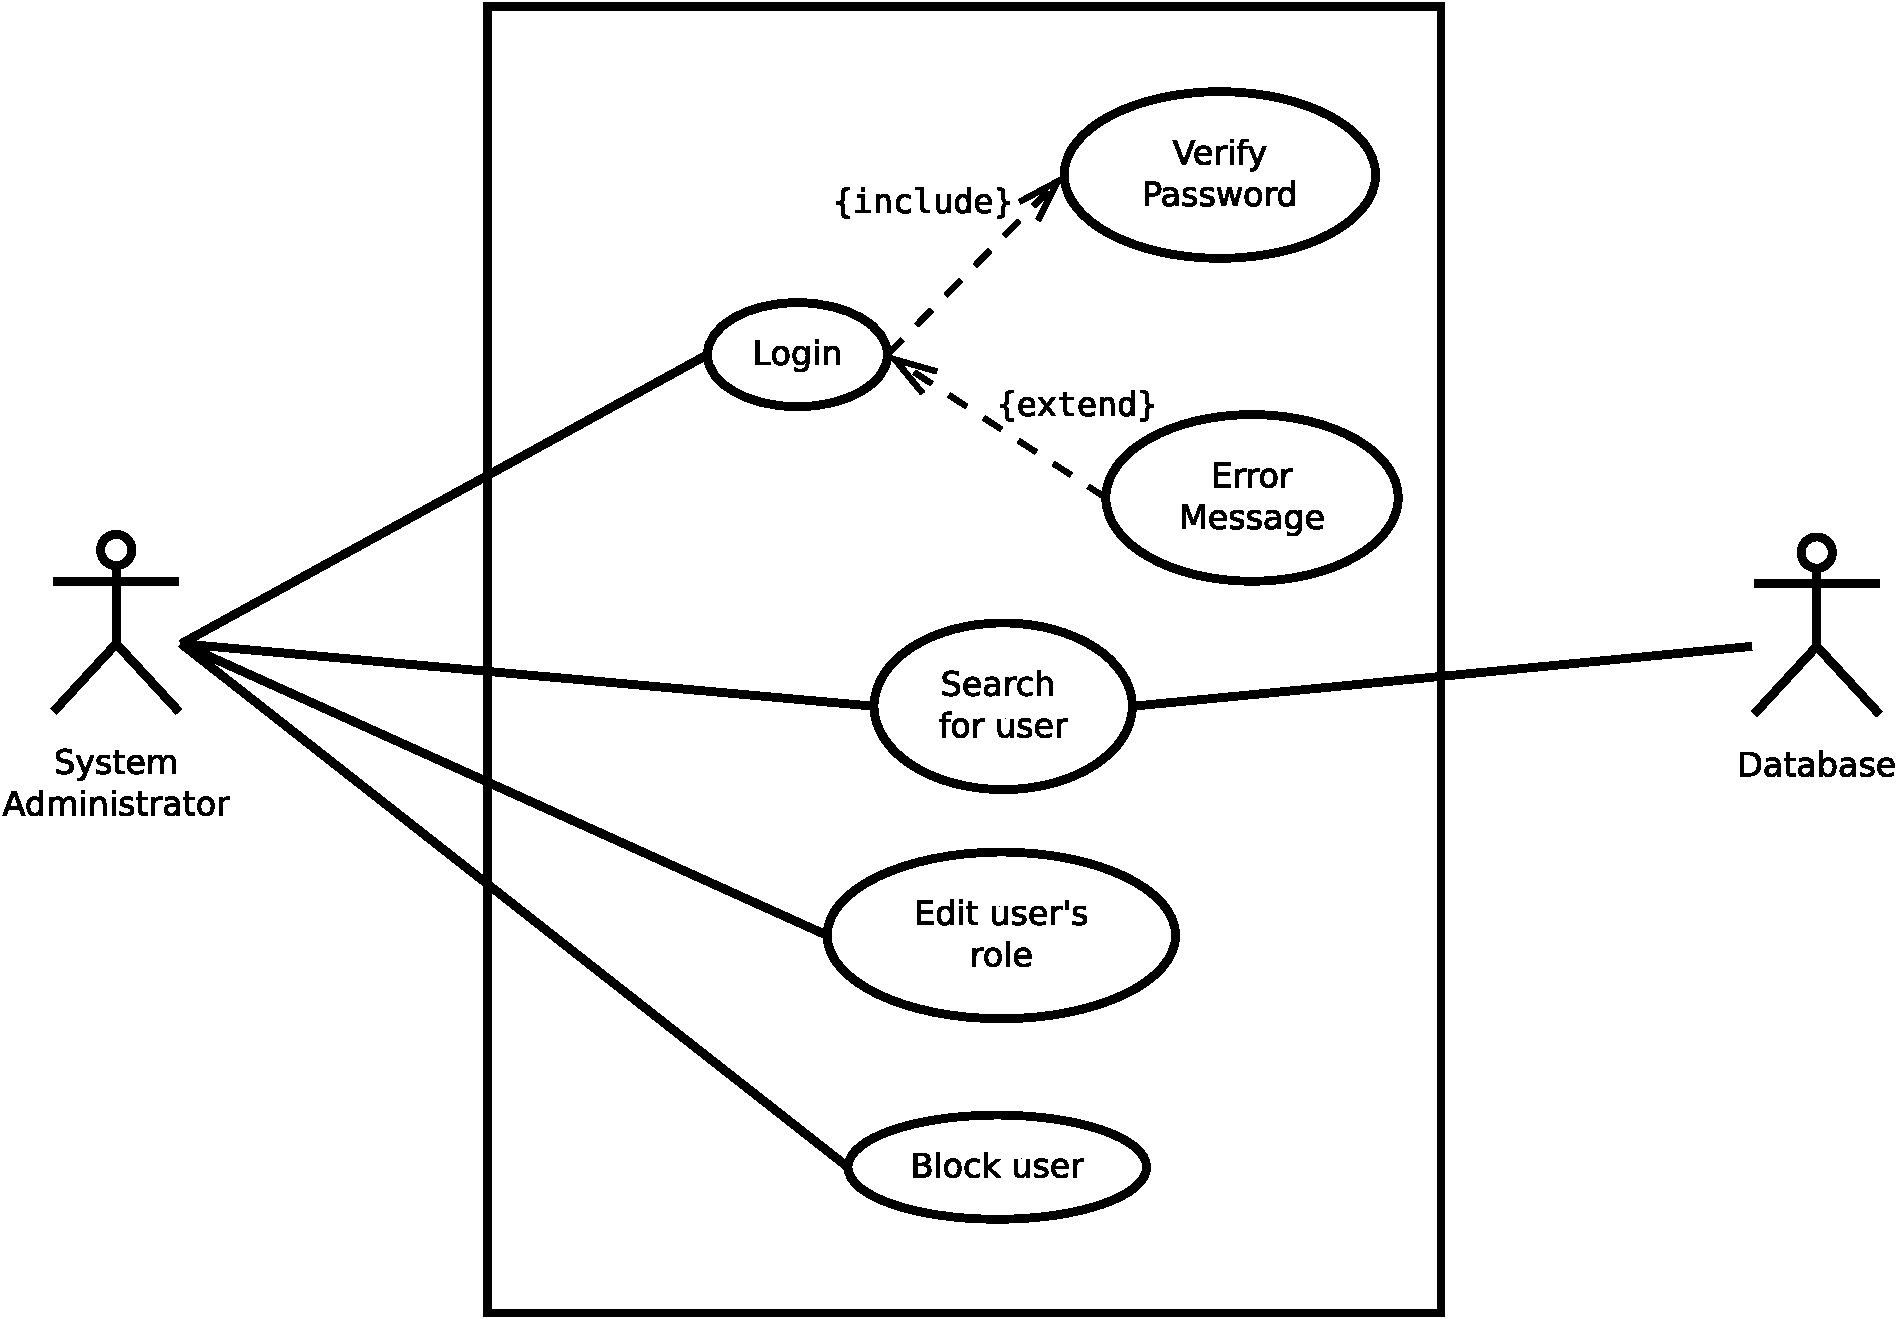
\includegraphics[scale=0.4,keepaspectratio=true]{./admin_use_case.pdf}
   \caption{Το use-case uml διάγραμμα της αλληλεπίδρασης του διαχειριστή συστήματος με την πλατφόρμα του παρατηρητήριο τιμών.}
    \label{uml2}
\end{figure}

\section{Αναφορές - πηγές πληροφοριών}
N/A

\section{Διαχειριστικές απαιτήσεις επιχειρησιακού περιβάλλοντος}

\subsection{Επιχειρησιακό μοντέλο}

\hspace{0.6cm}Η ικανοποίηση των χρηστών είναι απαραίτητη προύπόθεση για την επιτυχία του συστήματος.
Λόγω του ότι είναι άμεσος ο ρόλος των χρηστών εθελοντών κάνει την πλατφόρμα ελκυστική. Τους δίνεται ευκαιρία να ελέγχουν το περιεχόμενο και να ξέρουν ότι τα δεδομένα που βλέπουν είναι έγκυρα. Έτσι τους παρέχεται ένας τρόπος να πάρουν πληροφορίες που θα συνεισφέρουν στη λήψη αποφασεών που είναι πιο συμφέρουσες για μία αγορά. 

\hspace{0.6cm}Η εφαρμογή θα διαδοθεί από χρήστη σε χρήστη ως ένα εργαλείο σχεδιασμένο κυρίως για αυτούς και θα εγκαθιδρυθεί ως ένας βολικός τρόπος έρευνας αγοράς μέσω της συσκευής τους (desktop, tablet, κινητό). Χάρη σ'αυτή θα γλιτώνουν χρόνο αφού δεν θα χρειάζεται να σπαταλάνε ώρες στο δρόμο ψάχνοντας.

\subsection{Περιβάλλον διαχείρισης πληροφοριών}
\hspace{0.6cm}Διαχείριση πληροφοριών είναι η συλλογή και διαχείριση πληροφορίας από διάφορες πηγές και η προσφορά της σε διάφορα κοινά. Ο όρος κοινό περιλαμβάνει τα εμπλεκόμενα μέρη της εφαρμογής διαχείρισης της πληροφορίας και οποιονδήποτε άλλο έχει δικαίωμα πρόσβασης σε αυτή. Ως διαχείριση ορίζεται η οργάνωση και ο έλεγχος στη δομή, την επεξεργασία και διανομή της πληροφορίας.

\hspace{0.6cm}Άρα η διαχείριση πληροφοριών επικεντρώνεται στην ικανότητα ενός οργανισμού να συλλέξει, διαχειριστεί, διατηρήσει, αποθηκεύσει και διανείμει τη σωστή πληροφορία στους σωστούς ανθρώπους, την κατάλληλη στιγμή.

\hspace{0.6cm}Με βάση τη σημερινή εικόνα η διαχείριση πληροφοριών πρέπει να υιοθετεί και να προσκολάτε στις εξής καθοδηγητικές αρχές:
\begin{itemize}
 \item Κάθε αντικείμενο πληροφορίας είναι περιουσιακό στοιχείο της εταιρείας στην οποία ανήκει η πλατφόρμα που το διατηρεί και διαχειρίζεται.
 \item Κάθε πληροφορία της πλατφόρμας πρέπει να είναι διαθέσιμη και να μοιράζεται. Προφανώς δεν γίνεται όλες οι πληροφορίες που διατηρεί η πλατφόρμα να είναι διαθέσιμες προς όλους, για παράδειγμα ευαίσθητες πληροφορίες χρηστών όπως τα passwords. Αλλά κατά γενικό κανόνα πρέπει οι γενικές πληροφορίες να είναι διαθέσιμες προς όλους γιατί προάγει την χρήση της πλατφόρμας και την εκμετάλευση επιχειρηματικής γνώσης.
 \item Η διαχείριση και διατήρησης κάθε πληροφορίας που πρέπει να κρατά πλατφόρμα γίνεται εταιρικά. Αποθηκεύεται και διατηρείται η πληροφορία, δηλαδή ό,τι προσθέτει ο χρήστης τη μία μέρα πρέπει να υπάρχει και την επόμενη.
\end{itemize}

\hspace{0.6cm}Κάθε μέλος της εταιρείας που διαχειρίζεται και συντηρεί την πλατφόρμα είναι υπεύθυνο για την τήρηση των παραπάνω.

\section{Λειτουργικές απαιτήσεις επιχειρησιακού περιβάλλοντος}
\subsection{Επιχειρησιακές διαδικασίες}
\hspace{0.6cm}Οι διαχειριστές θα μπορούν να επεξεργάζονται τους λογαριασμούς των χρηστών προκειμένου να αλλάζουν τα δικαιώματα και τους ρόλους τους, μέσα από συγκεκριμένη σελίδα. Επίσης, θα έχουν τη δυνατότητα να διαγράφουν εθελοντές-χρήστες ή να αναστέλλουν την δυνατότητά τους για προσθήκη περαιτέρω προϊόντων, σε περίπτωση που δεν συμμορφώνονται με τους όρους χρήσης ή τα στοιχεία που εισάγουν είναι ανακριβή και ψευδή.

\subsection{Περιορισμοί}
\hspace{0.6cm}Οι διαχειριστές δεν έχουν εν γένει περιορισμούς στη διαχείριση του συστήματος και των δεδομένων, εκτός από το γεγονός ότι δεν θα μπορούν να βλέπουν ή να εντοπίζουν με κάποιον τρόπο τους κωδικούς των εγγεγραμμένων χρηστών.

\subsection{Δείκτες ποιότητας}
\hspace{0.6cm}Δείκτες ποιότητας είναι η αξιοπιστία, η αποδοτική επίδοση, η ασφάλεια, η συμβατότητα με άλλα συστήματα, η συντηρησιμότητα και η φορητότητα.

\hspace{0.6cm}Η επίδοση ενός συστήματος είναι σχετική με τους πόρους που μπορούν να χρησιμοποιηθούν σε κάθε κατάσταση στην οποία μπορεί να βρεθεί το σύστημα. Το σύστημα που προσφέρουμε πρέπει να είναι γρήγορα αποκρίσιμο. 

\hspace{0.6cm}Συμβατότητα είναι ο βαθμός με τον οποίον το σύστημα μας μπορεί να ανταλλάξει πληροφορίες με άλλα συστήματα και να εκτελέσει συγκεκριμένες λειτουργίες ενώ μοιράζονται το ίδιο υλικό. Είναι σημαντικό το συστημά μας να είναι συμβατό με εργαλεία διαγνωστικά και συντήρησης που θα χρησιμοποιούν οι διαχειριστές.

\hspace{0.6cm}Η χρηστικότητα είναι ο βαθμός στον οποίο το σύστημα μας μπορεί να χρησιμοποιηθεί από τους διαχειριστές για να πετύχουν τους στόχους τους με τρόπο αποτελεσματικό, αποδοτικό και ικανοποιητικό. Οι διαχειριστές πρέπει να μπορούν εύκολα να πραγματοποιούν τις ενέργειες που επιθυμούν μέσω πράξεων που είναι προφανής ο τρόπος που γίνονται.

\hspace{0.6cm}Το σύστημα πρέπει επίσης να είναι αποκρίσιμο και να ενημερώνει για τις λειτουργίες που εκτελεί κάθε στιγμή με σαφή τρόπο. Θα πρέπει να εμφανίζει πλήρως κατανοητά μηνύματα σφάλματος, για να μπορεί ο διαχειριστής να τα αντιμετωπίζει. 

\hspace{0.6cm}Τέλος θα πρέπει το σύστημα να μπορεί να επανέλθει μετά από σφάλματα διατηρώντας αντίγραφα ασφαλείας. 

\section{Έκθεση απαιτήσεων χρηστών}

\hspace{0.6cm}Οι διαχειριστές συστήματος απαιτούν να έχουν άνετη πρόσβαση μέσω της πλατφόρμας στο backend σύστημα για να διαχειρίζονται τους λογαριασμούς των χρηστών. Θέλουν να έχουν πρόσβαση στους λογαριασμούς κάθε χρήστη και να μπορούν να τους επεξεργαστούνν, να αλλάζουν τους ρόλους των χρηστών και να μπλοκάρουν χρήστες που θεωρούν ότι βλάπτουν την καλή λειτουργία του συστήματος και την ασφάλεια των άλλων χρηστών. 

\section{Αρχές του προτεινόμενου συστήματος}

Το προτεινόμενο σύστημα θα έχει τις εξής λειτουργικές αρχές:
\newline
\begin{enumerate}
 \item Δυνατότητα εισόδου ως διαχειριστής δίνοντας username και password.
 \item Δυνατότητα ανάκτησης password σε περίπτωση που ο διαχειριστής το ξέχασε.
 \item Δυνατότητα αναζήτησης λογαριασμών χρηστών μέσω μπάρας αναζήτησης.
 \item Δυνατότητα επισκόπησης των στοιχείων των λογαριασμών χρηστών με τη μορφή πίνακα.
 \item Δυνατότητα επεξεργασίας του ρόλου κάθε χρήστη μέσω κουμπιού edit.
 \item Δυνατότητα μπλοκαρίσματος/διαγραφής κάποιου χρήστη με χρήση κουμπιού διαγραφής.
\end{enumerate}

\newpage
\textbf{Σενάριο 1-Αλλαγή ρόλων χρηστών}
\begin{enumerate}
 \item  Ο διαχειριστής ανοίγει την αρχική σελίδα και κάνει login χρησιμοποιώντας το email και τον κωδικό του.
 \item Αν εισάγει λάθος password εμφανίζεται μήνυμα αποτυχίας και του δίνεται η δυνατότητα να ξανά εισάγει το password ή να πατήσει ότι το ξέχασε και να εκκινήσει διαδικασία ανάκτησης.
 \item Μετά την επιτυχή σύνδεση, οδηγείται σε σελίδα όπου μπορεί να δει όλα τα προφίλ των χρηστών σε βολική μορφή, καθένα από τα οποία θα έχει κάποιες επιλογές, μέσω κατάλληλων κουμπιών, για διαγραφή χρήστη ή αλλαγή ρόλων χρήστη. 
 \item Στην ίδια σελίδα υπάρχει μπάρα αναζήτησης για να βρίσκει γρήγορα συγκεκριμένους χρήστες.
 \item Έτσι θα μπορεί να διαγράψει κάποιον χρήστη αν οι πράξεις του δεν συνάδουν με τους όρους χρήσης της εφαρμογής ή αν συμπληρώνει αναληθή δεδομένα, μέσω κουμπιού διαγραφής χρήστη. Επίσης, θα μπορεί να αλλάξει τον ρόλο κάποιου χρήστη και να τον κάνει π.χ. και αυτόν διαχειριστή, σε περίπτωση που το κρίνει χρήσιμο, μέσω κουμπιού αλλαγής ρόλου χρήστη.
\end{enumerate}

\section{Περιορισμοί στο πλαίσιο του έργου}
Ν/Α

\section{Παράρτημα: ακρωνύμια και συντομογραφίες}




\end{document}
